%!TEX root = ../crimson_throne_book_main.tex
% 2015-08-22
Travelling to the Copper-Beater hall sends the party through the heart of the emperor's district again. They pass four of Pilts' ruffians on the way, who glare at the heroes and start chuckling, but do not engage. As the thugs walk down the street, a gaunt man with a blank stare in his eyes exits from an alleyway. He's clinging a simple wood-chopping axe in his grasp and is dressed in an ill-fitting and awkwardly strapped leather armor. The man pays the companions no heed, but trots off after the four bullies instead. Quint shouts out to him, but his cry only makes the emperor's men look back and notice the haggard man approaching. The wretch raises his axe and charges the thugs, but his inept swing goes wide and the next moment he is on the ground with the four ruffians on top of him. They cheerfully disarm the poor man and drag him along.\\

\hyperref[fig:Copper-beater-hall-Korvosa-555420262]{ The Copper-Beater Hall is an impressive structure } with a fancy front door. Peeking through the windows Puk makes out a luxurious meeting room and a richly decorated office, which are both deserted. The side of the building sports large warehouse doors through which crates and containers are normally transported in and out of the building, but they are shut now. The three chimneys are spouting black smoke, but there is no thunder of pounding hammers, which usually resounds from within. There is a third way in on the backside of the factory, which looks like the entrance for the workers. This is the entry point the companions choose. \\

\begin{figure}[h]
	\centering
	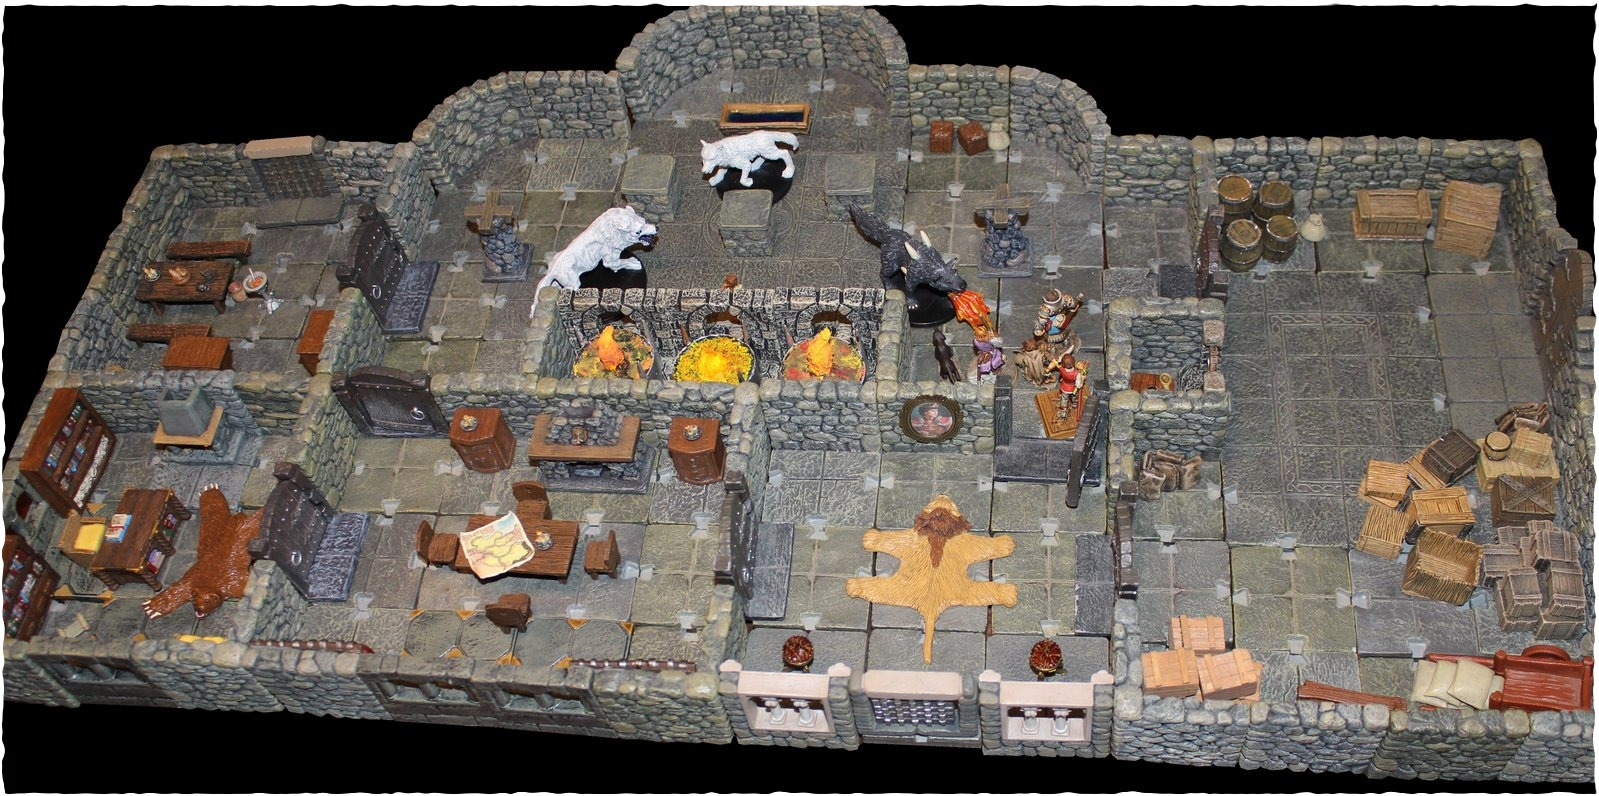
\includegraphics[width=0.4\textwidth]{images/Copper-beater-hall-Korvosa-555420262_mod.jpg}
	\caption{Copper-beater hall Korvosa}
	\label{fig:Copper-beater-hall-Korvosa-555420262}
\end{figure}

The heroes walk into a small changing room with some clothes and leather aprons hanging from pegs on the far wall. The dry, mouldy bread on the table suggests that the workers have not been here for some time. The door leading to the copper-beating furnaces feels slightly warm to the touch and Puk's observant ears pick up some low growls on the other side. Sjo casts {\itshape resist fire} on Balian and Puk, trusting that his innate fire resistance and Quint's ring will prove enough protection to withstand any potential fire attacks. As Balian pulls open the door, he is met by three powerfully built wolves, the size of draft horses, with ebony fur and fiery eyes. Spikes protrude from the fur on their backs which seems to flicker with red flames. The biggest of these hellhounds turns towards the intruders and spews forth a sea of flames, engulfing all companions in an inferno. His breath weapon also lights up oil which flows through several gutters in the workplace. Tied up in front of the blazing furnaces is Heldrin, who is now struggling to avoid the wall of fire that spreads through the room. Puk can evade the fire breath completely, while Quint and Balian get seared moderately. It is the fire-loving Shoanti, however, who takes a heavy burn. Before he can recover, Sjo gets jumped by a second warhound, whose fierce bite puts him down. Quint pulls Spyder, who is also heavily charred, behind the open door and waits for Puk and Balian to lure the hellish canine into the changing room. Then he kicks the door shut, giving his friends the opportunity to quickly take out this opponent. Meanwhile the bard uses his wand to put Sjo back on his feet. \hyperref[fig:Facing-Nessian-Warhounds-in-Copper-Beater-Hall-555420948]{ Next Quint reopens the door and Balian charges the two remaining Nessian warhounds the workplace } . Through sheer luck Heldrin has avoided most of the flames and is still on his feet, though barely. Fortunately the oil in the gutters has burned away and the fire in the room is now dying out. Balian cleaves and Quint makes it to his side, for the ranger is taking multiple bites and is in desperate need of healing. Puk tumbles into an advantageous position and works his sneaking magic. Sjo aids in healing Balian, whose heavy hits kill off a second hound, but the ranger still gets dropped himself before his friend finish off the last Nessian warhound. \\

\begin{figure}[h]
	\centering
	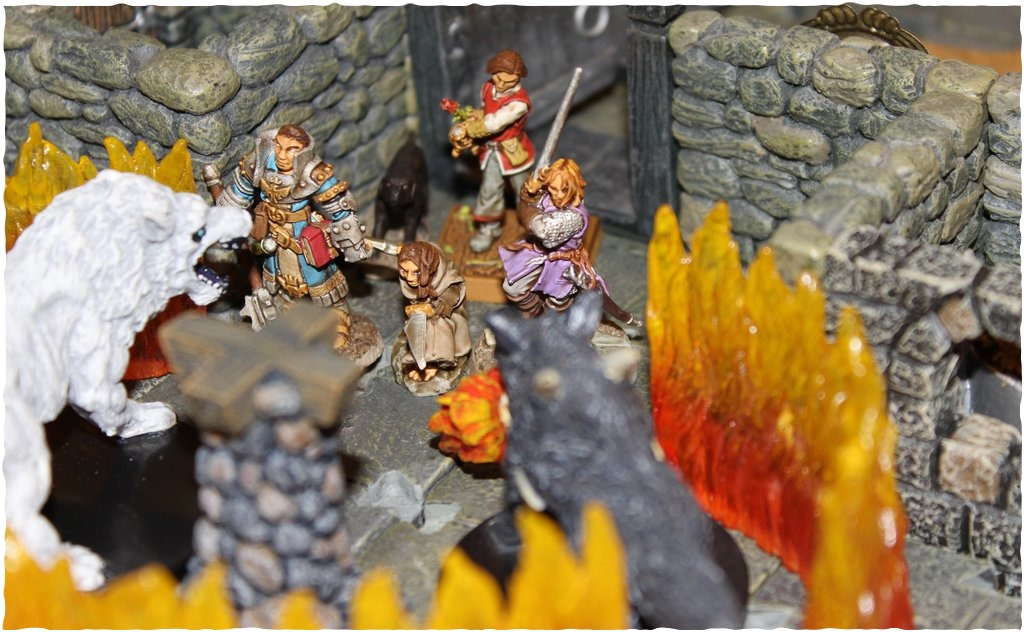
\includegraphics[width=0.4\textwidth]{images/Facing-Nessian-Warhounds-in-Copper-Beater-Hall-555420948_mod.jpg}
	\caption{Facing Nessian Warhounds in Copper-Beater Hall}
	\label{fig:Facing-Nessian-Warhounds-in-Copper-Beater-Hall-555420948}
\end{figure}

The healing wands are drained further of their {\itshape cures} and the companions realize they are slowly getting through their resources with at least one more rescue attempt ahead. Quint notices a wooden replica of the Old City Hall, the tall spire of which has in indentation which fits the feet of the Mouse miniature. At one time in history, this belfry-like structure was the tallest building in all of Varisia, until the Arvensoar in Magnimar stole away that distinction for more than a decade. Korvosa quickly reclaimed the honor with the completion of the north tower on Castle Korvosa, though. The Old City Hall's black stone walls have led to people calling it the Charcoal Palace. It served Korvosa as city hall for 60 years, until Remsev Ornelos decided that its many stairs leading up the tall tower were a terrible inconvenience to anyone working there. The building might have been prestigious in design, it was also very impractical. So when the city expanded to the mainland, the Korvosans constructed a new, more practical city hall in North Point, which remains in place until today. The Old City Hall has housed a handful of private initiatives over the last two centuries, but it has stood empty for at least as long as any of the companions can remember, serving mainly as a landmark in the oldest part of the city. Will this tall tower be the arena for the party's confrontation with Alika and Rolth? Judging by their resources, the heroes certainly hope so. 